
\section{Moving to the Cloud}

\begin{frame}{OpenShift}
\textbf{OpenShift} is an open-source container system from
\textbf{Red Hat}. It supports \textit{Docker} containers natively using
\textit{Kubernetes} (a container \textit{orchestrator} from Google).

OpenShift can be used both \textit{on-premise} (even for free) or
\textit{online} (using Red Hat's own cloud).

OpenShift enables \textit{Platform-as-a-Service} cloud.

\centering
\vspace{1em}

\includegraphics[keepaspectratio=true,height=40pt]{openshift_logo}
\hspace{1em}

\includegraphics[keepaspectratio=true,height=40pt]{docker_logo}
\end{frame}


\begin{frame}{OpenShift}
\centering
\hspace*{-0.4in}
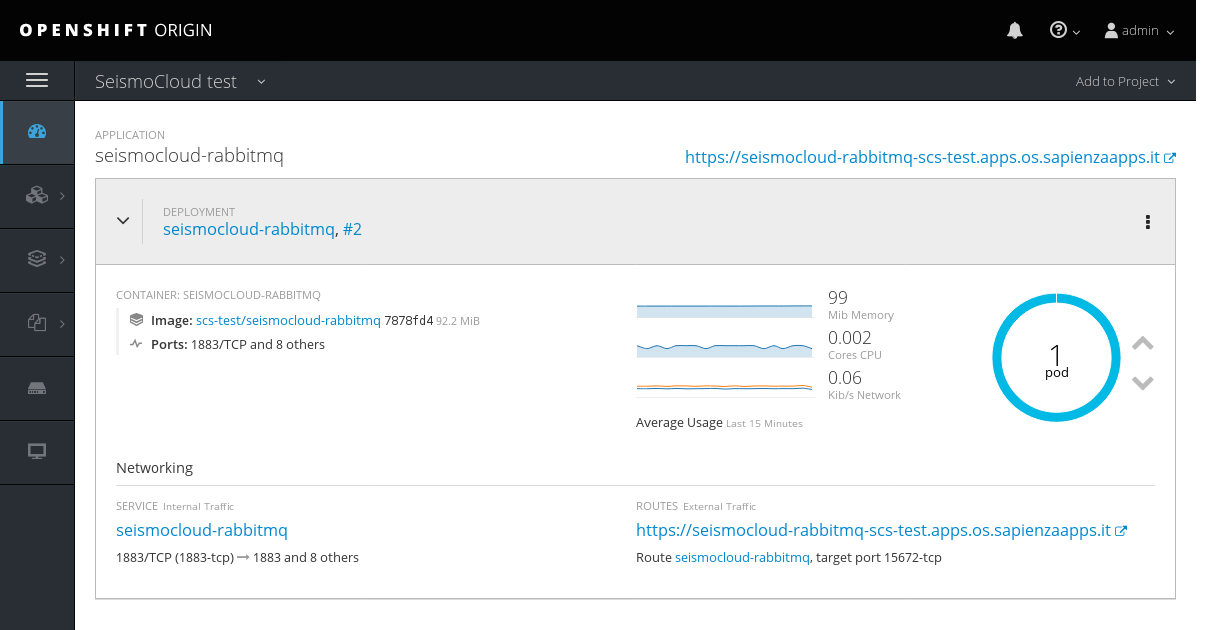
\includegraphics[width=1.19\textwidth]{openshift}
\end{frame}


\begin{frame}{PaaS advantages}
By deploying this project on Red Hat's OpenShift cloud, we have:

\begin{itemize}
  \item \textbf{High availability}: Red Hat has many datacenter, and OpenShift
  is capable to power up pods in different sites around the globe. Also it uses
	Amazon AWS to load-balacing its own servers (\textit{Hybrid IaaS}).
  \item \textbf{High elasticity}: the underlying Kubernetes is able to scale
  automatically based on resource usages (eg. CPU/memory) and/or external
	triggers (such as the application itself)
	\item \textbf{Pay-per-use}: we'll pay per-use, so costs will grow as the user
	base grow, and we'll be able to react to usage peaks (earthquakes)
\end{itemize}
\end{frame}




\begin{frame}{PaaS multi-tiering}

By using Docker we'll be able to have a \textbf{multi-tier} architecture:
many cloud providers supports Docker containers (such as Amazon EC2, Google
Cloud, IBM Bluemix) as a backup, load balacing or as new main cloud provider in
the future, with no changes to the code.

\begin{center}

\includegraphics[width=0.5\textwidth]{amazon_ec2}
\end{center}


In fact, in this (\textit{testing}) phase, we have an hybrid cloud system:
we have both \textit{on-premise} and \textit{on-cloud} OpenShift instances, and
some plain Docker containers in the production server \textbf{deployed with the
same Docker images}.

\end{frame}



\begin{frame}{Old vs PaaS: costs and SLA}

Recap of conditions for the current architecture:

\begin{itemize}
  \item \textbf{Costs (yearly)}: \circa 1400 €
  \item \textbf{SLA} (server+net): 99.00\% (\circa 7.5 hours per month)
  \item \textbf{Maintenance}: software/O.S. maintenance is our duty
  \item \textbf{No HA, no scalability, no redundancy}
\end{itemize}

With OpenShift \textit{Platform-as-a-Service} and new architecture:

\begin{itemize}
  \item \textbf{Costs (yearly)}: \circa 1000 € at \textbf{idle}, plus
	\textbf{one-time cost} of 7500 €
  \item \textbf{SLA} (PaaS+net): from 99.00\% to 99.99\% (\circa 4 minutes)
  \item \textbf{Maintenance}: software/O.S. maintenance is offloaded
  to the PaaS provider - we need to maintain only our own software
  \item \textbf{HA, scalability, elasticity, ...}
\end{itemize}

\end{frame}
